\documentclass[a4paper,12pt]{article}
\usepackage[margin=1in]{geometry}

\usepackage[T2A]{fontenc}			% кодировка
\usepackage[utf8]{inputenc}			% кодировка исходного текста
\usepackage[english,russian]{babel}	% локализация и переносы
\usepackage{graphicx}                % Математика
\usepackage{amsmath,amsfonts,amssymb,amsthm,mathtools} 
\usepackage{mathtext}
\usepackage[T2A]{fontenc}
\usepackage[utf8]{inputenc}

\usepackage{wasysym}

%Заговолок
\author{Бичина Марина 
группа Б04-005 1 курса ФЭФМ}
\title{}
\date{}


\begin{document} % начало документа

\begin{center}
\begin{Large}
{ Марина Б04-005, Лабораторная работа №.3.4.4: Петля гистерезиса (статический метод)}
\end{Large}
\end{center}
\paragraph{Цель работы:} 
\begin{enumerate}
\itemsep0em
\item Исследование основной кривой намагничивания и предельной петли гистерезиса для образца тороидальной формы, изготовленного из стали
\end{enumerate}
\paragraph{Оборудование:}
\begin{enumerate}
\itemsep0em
\item источник питания
\item тороид
\item соленоид
\item баллистический гальванометр с осветителем и шкалой 
\item амперметр
\item лабораторный автотрансофрматор
\item разделительный трансформатор 
\end{enumerate}

\paragraph{Теоретическая справка:}

Магнитная индукция \textbf{В} и напряженность поля \textbf{Н} в ферромагнетике связаны неоднозначно, поскольку магнитная восприимчивость $\chi$ не является константой и зависит от \textbf{Н}, при этом, индукция еще зависит и от предыстории образца. 
\paragraph{} Данное явление несет название "гистерезис". Связь между \textbf{В}и \textbf{Н} в типичном ферромагнетике иллюстрирует рисунок \ref{plot_theory}.
\begin{figure}[h]
\centering
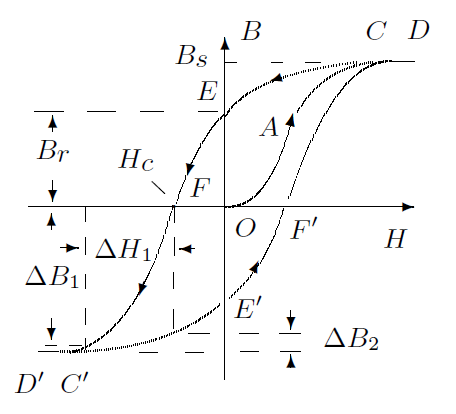
\includegraphics[scale=0.5]{plot_theory.png}
\caption{Петля гистерезиса ферромагнетика (теоретическая)}
\label{plot_theory}
\end{figure}

\paragraph{} \textbf{Формулы, необходимые для подсчетов:\\}
Связь напряженности магнитного поля в тороиде от тока
\begin{equation}
H \approx \frac{N}{\pi\cdot D}I
\end{equation}
Формула, необходимая для нахождения изменения магнитной индукции, после выражения баллистической постоянной 
\begin{equation}
\Delta B = \mu_0 \cdot N_{c} \cdot \frac{N^{'}_{c}}{N^{'}} \frac{R}{R_{c}}\frac{d_{c}^2}{d^2} \frac{\Delta I_{c}}{l_{c}} \frac{\Delta x}{\Delta x_{c}}
\end{equation}
где:
\begin{enumerate}
\itemsep0em
\item $\mu_0 = 1.257 \cdot 10^{-6} \frac{\text{Гн}}{\text{м}}$ - магнитная постоянная
\item $N = 1750, N_{c} = 940\;\;N^{'}_{c} = 500\;\;N^{'} = 300$, - число витков у намагничивающейся обмотки, пустотелого соленоида, измерительной катушки, тороида
\item $R = R_{c}$ - полное сопротивление измерительной цепи тороида, полное сопротивление измерительной цепи соленоида
\item $D = 10 \text{см}, d_c =7\text{см} \;\; d = 1\text{см}$ - диаметры тора, соленоида и сердечника
\item $\Delta I_{c} = 1706 \text{мА}$ - ток, проходящий через соленоид
\item $l_{c} = 80\text{см}$ - длина соленоида 
\item $\Delta x\;\; \Delta x_{c} = 16$ - отклонения солнечного зайчика  на тороиде и соленоиде
\end{enumerate}
\paragraph{Описание установки:}
\paragraph{}
\begin{figure}[h!]
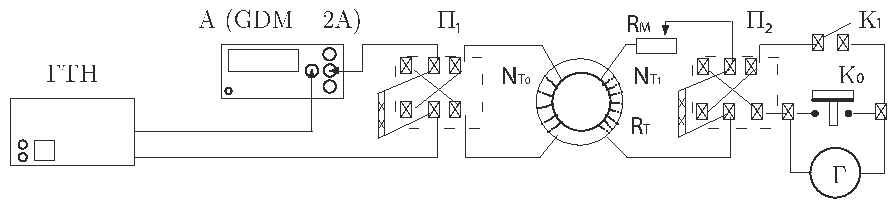
\includegraphics[scale=1]{ustanovka_1.pdf}
\caption{Схема установки для исследования петли гистерезиса}
\label{ustanovka_1}
\end{figure}
\paragraph{}
\begin{figure}[h!]
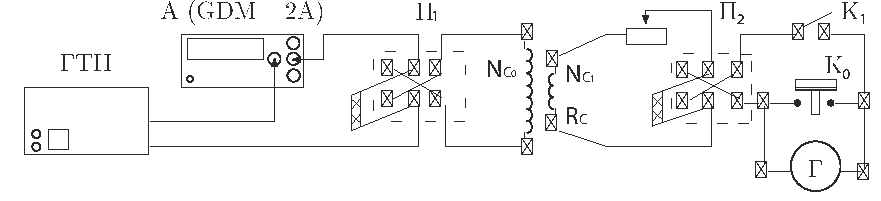
\includegraphics[scale=1]{ustanovka_2.pdf}
\caption{Схема установки для калибровки гальванометра}
\label{ustanovka_2}
\end{figure}
Все константы, связанные с установками, приведены выше
\paragraph{Ход работы:}
\begin{enumerate}
\itemsep0em
\item Посчитаем константы:\\
$\alpha = 55.7\;\;\text{1/м} \Rightarrow H = \alpha I$\\
$\beta = \mu_0 \cdot N_{c} \cdot \dfrac{N^{'}_{c}}{N^{'}} \dfrac{d_{c}^2}{d^2} \dfrac{1}{l_{c}}\dfrac{\Delta I_{c}}{\Delta x_{c}} \approx 0.0128\;\;\text{H/(A*см)} \Rightarrow \Delta B = \beta \cdot \Delta x$

\item Перенесем в таблицу данные, полученные при выполнении лабораторной работы:

\begin{table}[h!]
\centering
\begin{tabular}{|l|l|l|l||l||l|l|l|l|}
\hline 
I, мА  & $\Delta x$, см & H, А/м    & $\Delta B$, Тл &  &       &       &          &         \\
\hline 
61.8   & 3.8            & 344.226   & 48.64          &  & -436  & -32   & -2428.52 & -409.6  \\
124.3  & 9.1            & 692.351   & 116.48         &  & -623  & -50.2 & -3470.11 & -642.56 \\
175.68 & 15.8           & 978.5376  & 202.24         &  & -869  & -59.1 & -4840.33 & -756.48 \\
196.1  & 19.9           & 1092.277  & 254.72         &  & -1206 & -67.6 & -6717.42 & -865.28 \\
217.48 & 24.9           & 1211.3636 & 318.72         &  & -1705 & -74.7 & -9496.85 & -956.16 \\
237.21 & 31.7           & 1321.2597 & 405.76         &  & -1209 & -69.2 & -6734.13 & -885.76 \\
257.67 & 37.7           & 1435.2219 & 482.56         &  & -871  & -64   & -4851.47 & -819.2  \\
278.6  & 45.9           & 1551.802  & 587.52         &  & -623  & -58.5 & -3470.11 & -748.8  \\
307.2  & 56.1           & 1711.104  & 718.08         &  & -435  & -53   & -2422.95 & -678.4  \\
353.83 & 75.6           & 1970.8331 & 967.68         &  & -351  & -50.2 & -1955.07 & -642.56 \\
623    & 95.1           & 3470.11   & 1217.28        &  & -305  & -48.7 & -1698.85 & -623.36 \\
868    & 104.6          & 4834.76   & 1338.88        &  & -276  & -47.7 & -1537.32 & -610.56 \\
1204   & 114.1          & 6706.28   & 1460.48        &  & -255  & -46.9 & -1420.35 & -600.32 \\
1702   & 122.4          & 9480.14   & 1566.72        &  & -234  & -46.1 & -1303.38 & -590.08 \\
1200   & 117.1          & 6684      & 1498.88        &  & -214  & -45.3 & -1191.98 & -579.84 \\
868    & 110.3          & 4834.76   & 1411.84        &  & -193  & -44.5 & -1075.01 & -569.6  \\
623    & 104.3          & 3470.11   & 1335.04        &  & -173  & -43.7 & -963.61  & -559.36 \\
436.6  & 97.6           & 2431.862  & 1249.28        &  & -121  & -41.2 & -673.97  & -527.36 \\
353.8  & 95.3           & 1970.666  & 1219.84        &  & -60   & -37.7 & -334.2   & -482.56 \\
307    & 93.4           & 1709.99   & 1195.52        &  & 0     & -33.7 & 0        & -431.36 \\
278.6  & 92.4           & 1551.802  & 1182.72        &  & 60    & -28.2 & 334.2    & -360.96 \\
257.7  & 91.6           & 1435.389  & 1172.48        &  & 122   & -17.7 & 679.54   & -226.56 \\
237.21 & 90.8           & 1321.2597 & 1162.24        &  & 173   & -11.7 & 963.61   & -149.76 \\
217.48 & 90             & 1211.3636 & 1152           &  & 194   & -7.4  & 1080.58  & -94.72  \\
196.1  & 89.1           & 1092.277  & 1140.48        &  & 215   & -1.9  & 1197.55  & -24.32  \\
175    & 88.2           & 974.75    & 1128.96        &  & 2355  & 4.1   & 13117.35 & 52.48   \\
123    & 85.7           & 685.11    & 1096.96        &  & 256   & 12.3  & 1425.92  & 157.44  \\
60.9   & 82.2           & 339.213   & 1052.16        &  & 277   & 21.8  & 1542.89  & 279.04  \\
0      & 78.2           & 0         & 1000.96        &  & 306   & 35.3  & 1704.42  & 451.84  \\
-61.14 & 72.4           & -340.5498 & 926.72         &  & 352   & 58.3  & 1960.64  & 746.24  \\
-123   & 61.6           & -685.11   & 788.48         &  & 436   & 83.8  & 2428.52  & 1072.64 \\
-174   & 55.6           & -969.18   & 711.68         &  & 623   & 105.8 & 3470.11  & 1354.24 \\
-195   & 51.4           & -1086.15  & 657.92         &  & 870   & 114.3 & 4845.9   & 1463.04 \\
-216   & 46.3           & -1203.12  & 592.64         &  & 1208  & 123.3 & 6728.56  & 1578.24 \\
-236   & 40.1           & -1314.52  & 513.28         &  & 1708  & 130.8 & 9513.56  & 1674.24 \\
-257   & 32.2           & -1431.49  & 412.16         &  &       &       &          &         \\
-278   & 24             & -1548.46  & 307.2          &  &       &       &          &         \\
-306   & 11             & -1704.42  & 140.8          &  &       &       &          &         \\
-352   & -6.5           & -1960.64  & -83.2          &  &       &       &          &   \\
\hline      
\end{tabular}
\caption{Данные, полученные при обработки лабораторной работы}
\end{table}

\item По полученным данным построим график 
\begin{figure}[h!]
\centering
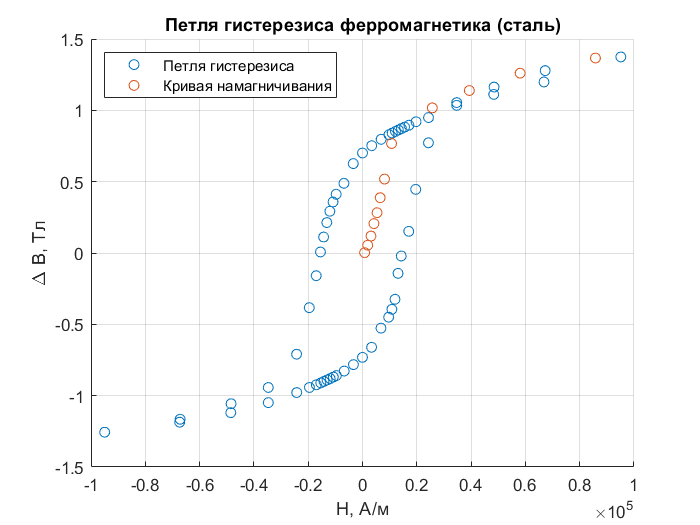
\includegraphics[scale=0.6]{plot.png}
\end{figure}
\item из графика найдем коэрцитивную силу $H_{c}$ и индукцию насыщения $B_{s}$:
\item рассчитаем максимальную дифференциальную магнитную проницаемость для начальной кривой намагничивания:
$\mu =\dfrac{1}{\mu_0} \dfrac{dB}{dH}\approx 422$ 
\item Построим сводную таблицу:

\begin{table}[h!]
\centering
\begin{tabular}{|l|l|l|l|}
\hline
                                                                      & $H_{s}$, A/м      & $ B_{s}$, Тл & $\mu$ \\ \hline
\begin{tabular}[c]{@{}l@{}}экспериментальные \\ значения 
\end{tabular} & $(1.50 \pm 0.01) \cdot 10^4 $ & $1.450 \pm 0.01$, Тл      & $420 \pm 20$   \\ \hline
\end{tabular}
\caption{Cводная таблица экспериментальных значений}
\end{table}
\end{enumerate}


\paragraph{Выводы:}
\begin{enumerate}
\item Мы нашли коэрцитивную силу $H_{c} = 1.500 \pm 0.01$ А/м и индукцию насыщения $B_{s} = 1.450 \pm 0.01$ Тл. (но по нашему графику не совсем корректно определять $B_{s}$, поскольку на нашем графике не прослеживается прямая, параллельная оси ОХ. Но мы можем определить остаточную индукцию, равную $B_r \approx 0.7$ Тл, что может помочь нам в определении типа стали)
\item Нашли дифференциальную магнитную проницаемость, равную $\mu = \dfrac{1}{\mu_0}\dfrac{dB}{dH} = 420 \pm 20$ 
\item Из эксперимента сложно определить, какой тип стали нам представлен. Наиболее вероятным из вариантов является сталь кобальтовая, относящаяся к магнитожестким ферромагнетикам. 
\end{enumerate}
\end{document}